\documentclass[tikz,border=10pt]{standalone}
\usetikzlibrary{calc}

\begin{document}
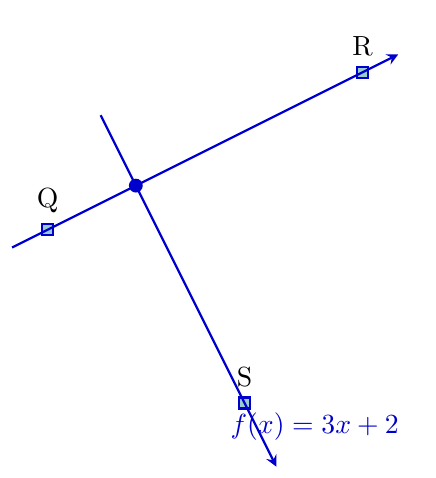
\begin{tikzpicture}[
  pt/.style={rectangle,draw=blue!80!black,fill=teal!40,inner sep=2pt,thick,label={#1},name=#1},
  extline/.style={thick,draw=blue!80!black,-stealth,shorten >=-#1,shorten <=-#1},
  extline/.default=1cm
]

\node [pt=Q] at (0,0) {};
\node [pt=R] at (4,2) {};
\node [pt=S] at (2.5,-2.2) {};

\draw [extline=0.6cm] (Q) -- (R);
\draw [extline] ($(Q)!(S)!(R)$) -- (S);

\fill [blue!80!black] ($(Q)!(S)!(R)$) circle [radius=2.5pt];

% Example math annotation:
\node[below right, blue!80!black] at (2.2,-2.2) {$f(x) = 3x + 2$};

\end{tikzpicture}
\end{document}